\begin{frame}{Matrix Evolution \tiny{(aside)}}
    Adjacency matrices are used in graph theory to encode a graph's structure.
    \begin{columns}
        \begin{column}{.3\textwidth}
            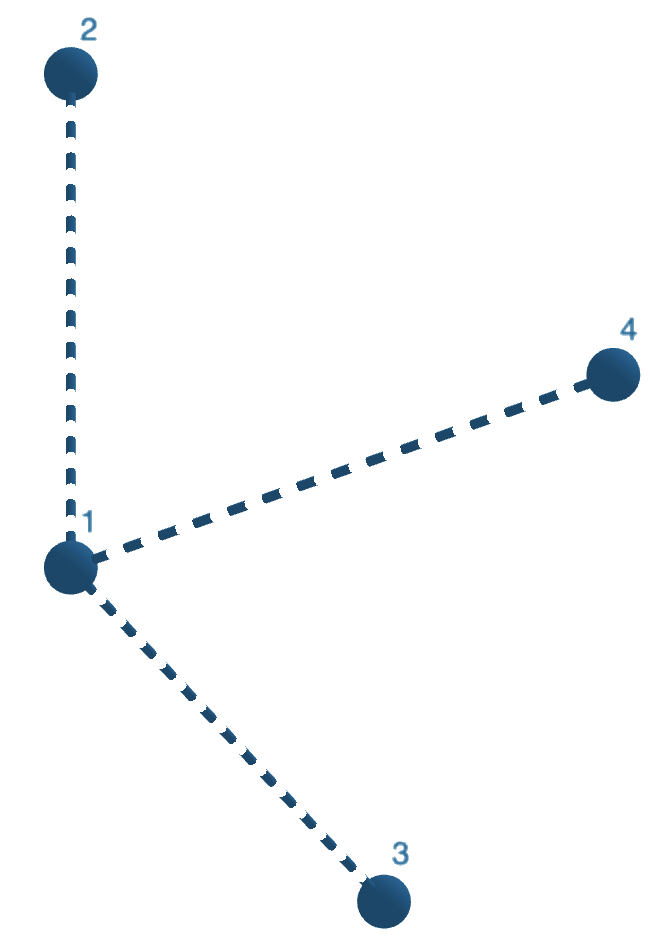
\includegraphics[width=.8\textwidth, clip=True, trim= 0in .05in 0in 0in]{../Images/my_graph.png}
        \end{column}        
        \begin{column}{.7\textwidth}
            Adjacency $\Ria$ Discrete
            \begin{itemize}
                \item Distance: Integer number of Hops
                \item Connectivity: Integer Number of Paths
            \end{itemize}
            Affinity $\Ria$ $\sim$Continuous 
            \begin{itemize}
                \item Distance: Function Space Measurement 
                \item Connectivity: Encoded in $\mathbf{A}$ and ${\vec{\gamma}}$
            \end{itemize}
        \end{column}
    \end{columns} 
    \bc
        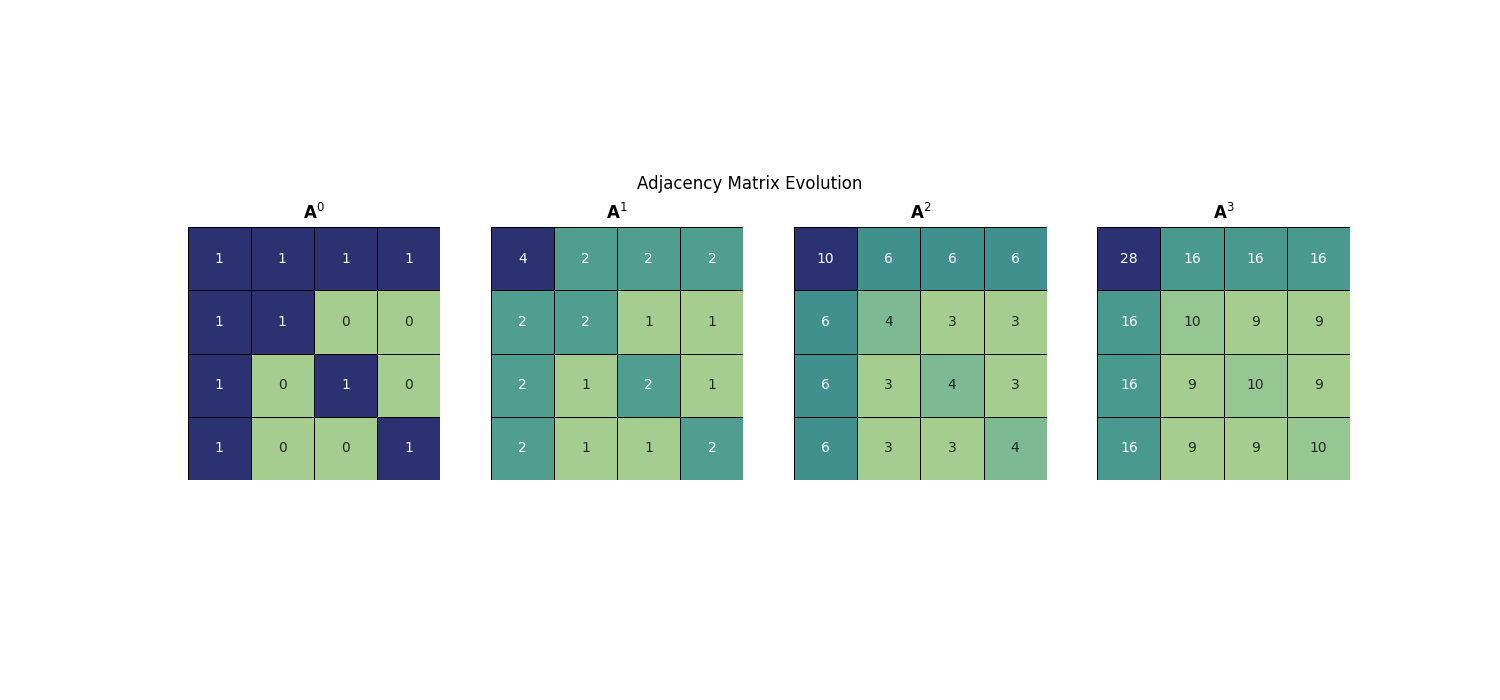
\includegraphics[width=.9\textwidth, clip=True, trim= 1.45in 2.15in 1.45in 1.75in]{../Images/matrix_evo.png}
    \ec    
\end{frame}

% \begin{frame}{Example Results and Reporting}
% Starting Splunk query refined with the analyst team:\\
% \begin{center}
%     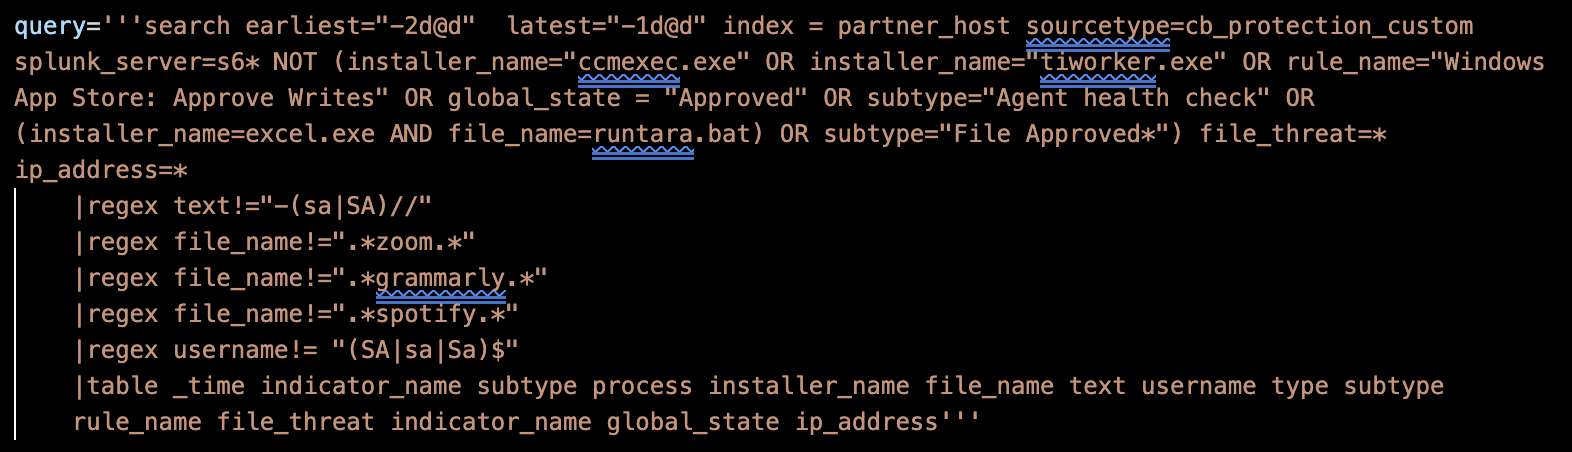
\includegraphics[width=\textwidth]{../Images/query.png}
% \end{center}

% \end{frame}

% \begin{frame}{Example Results and Reporting}
% HSI log for this query:\\
% \begin{center}
%     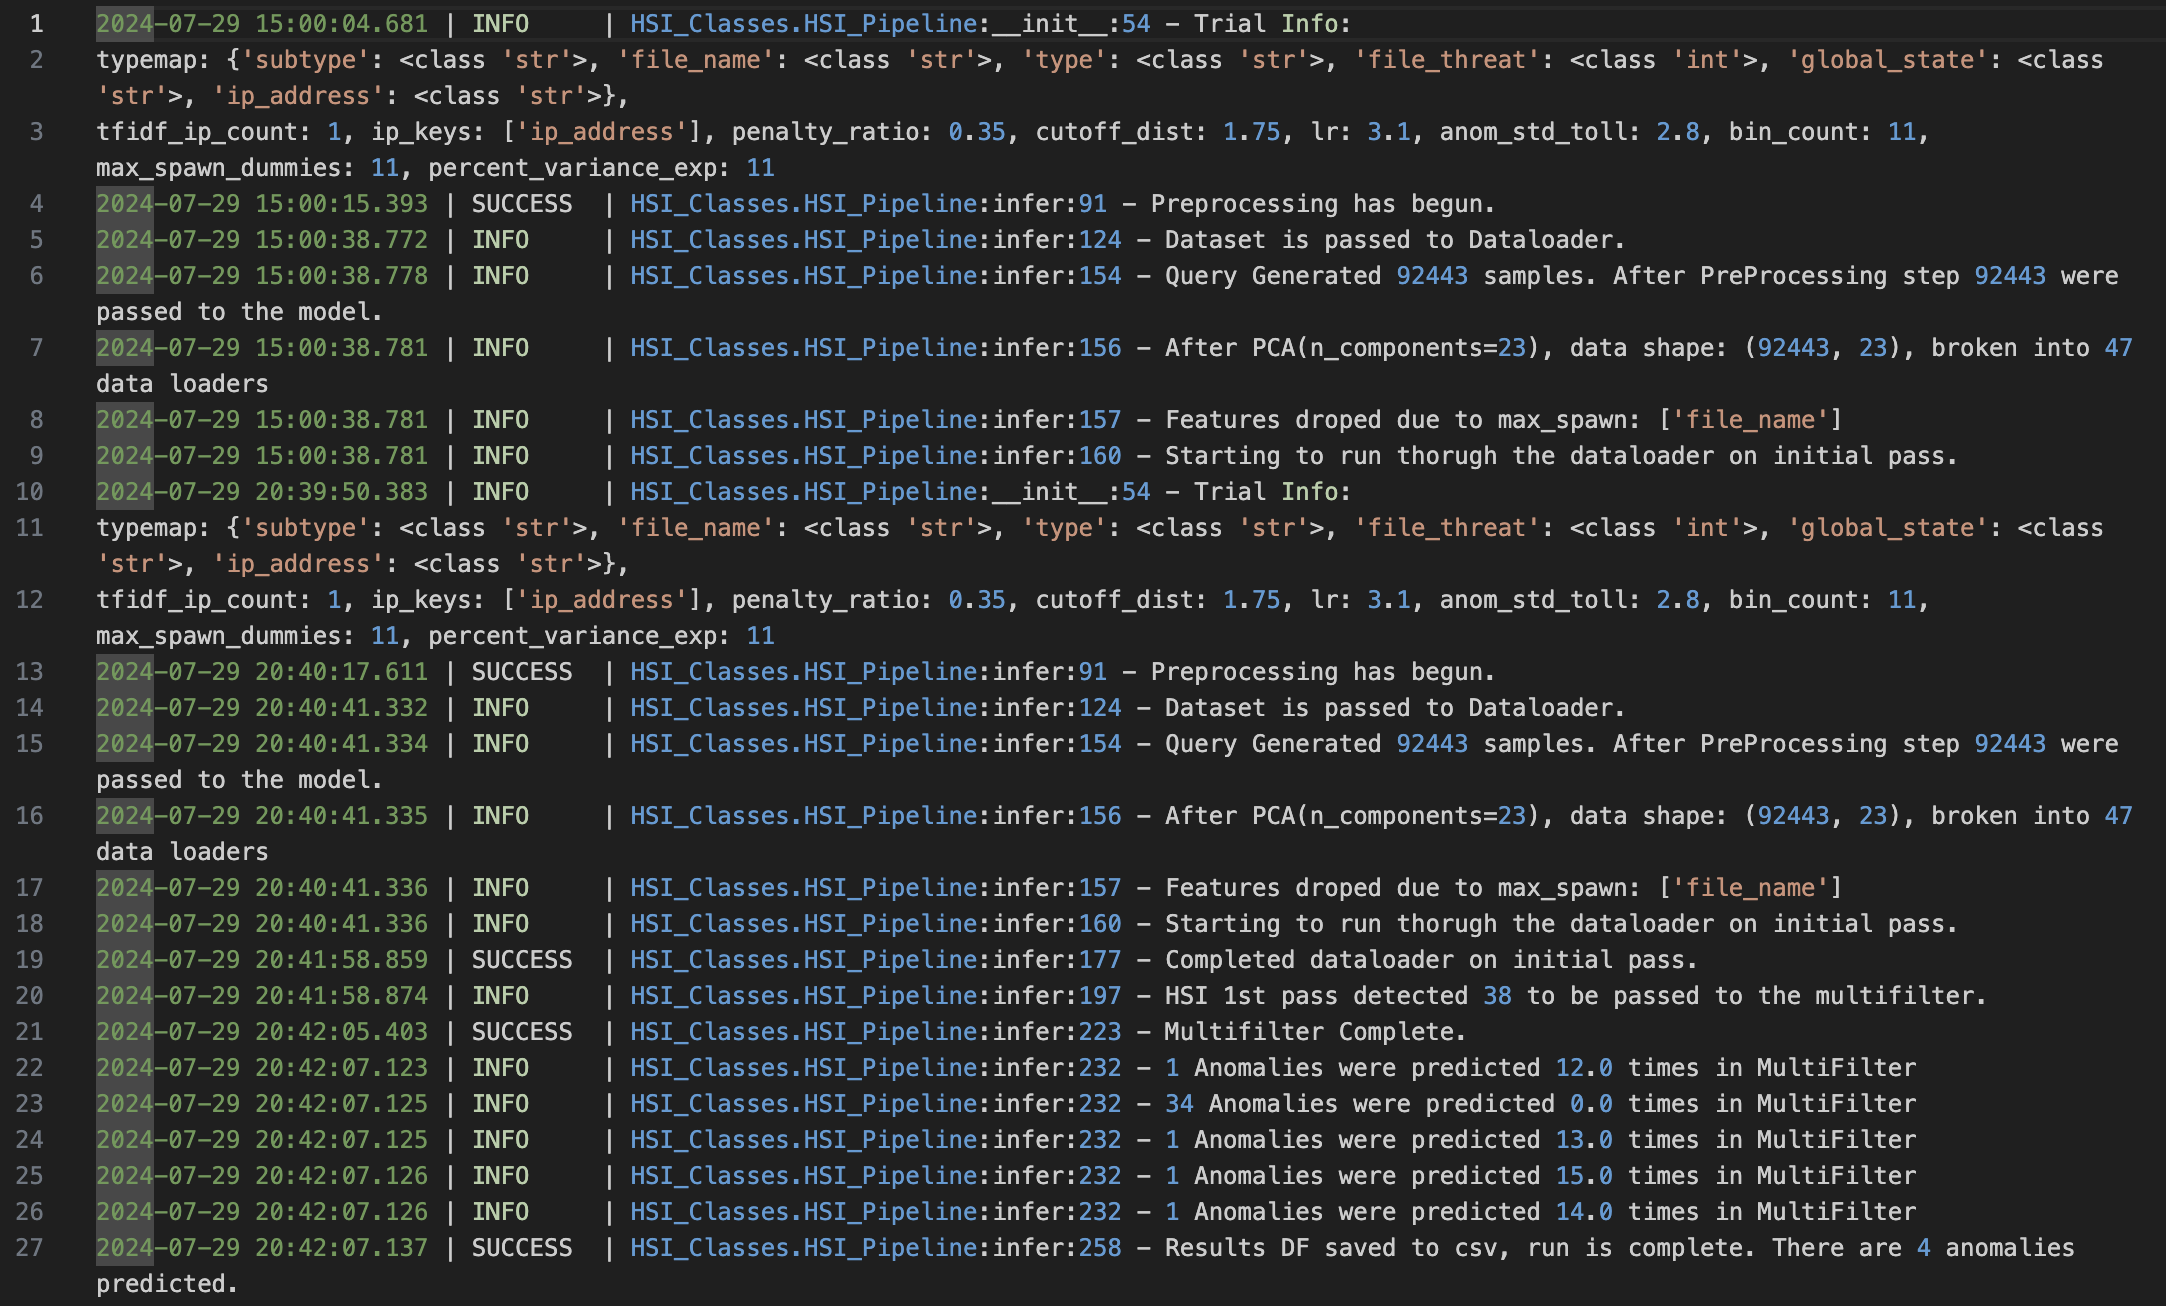
\includegraphics[clip=true, trim=.5in 0in 0in 3.3in, width=\textwidth]{../Images/Log.png}
% \end{center}


% We find:
% \begin{columns}
% \begin{column}{.5\textwidth}
% \begin{itemize}
%     \item 92,443 Events/Day
%     \item 38 Initial Predictions
% \end{itemize}
% \end{column}
% \begin{column}{.5\textwidth}
% \begin{itemize}
%     \item 34 False Positives
%     \item 4 Multifilter Anomalies  
% \end{itemize}
% \end{column}
% \end{columns}
% \end{frame}


% \begin{frame}{Example Results and Reporting}
% HSI results for this query:\\
% \begin{center}
%     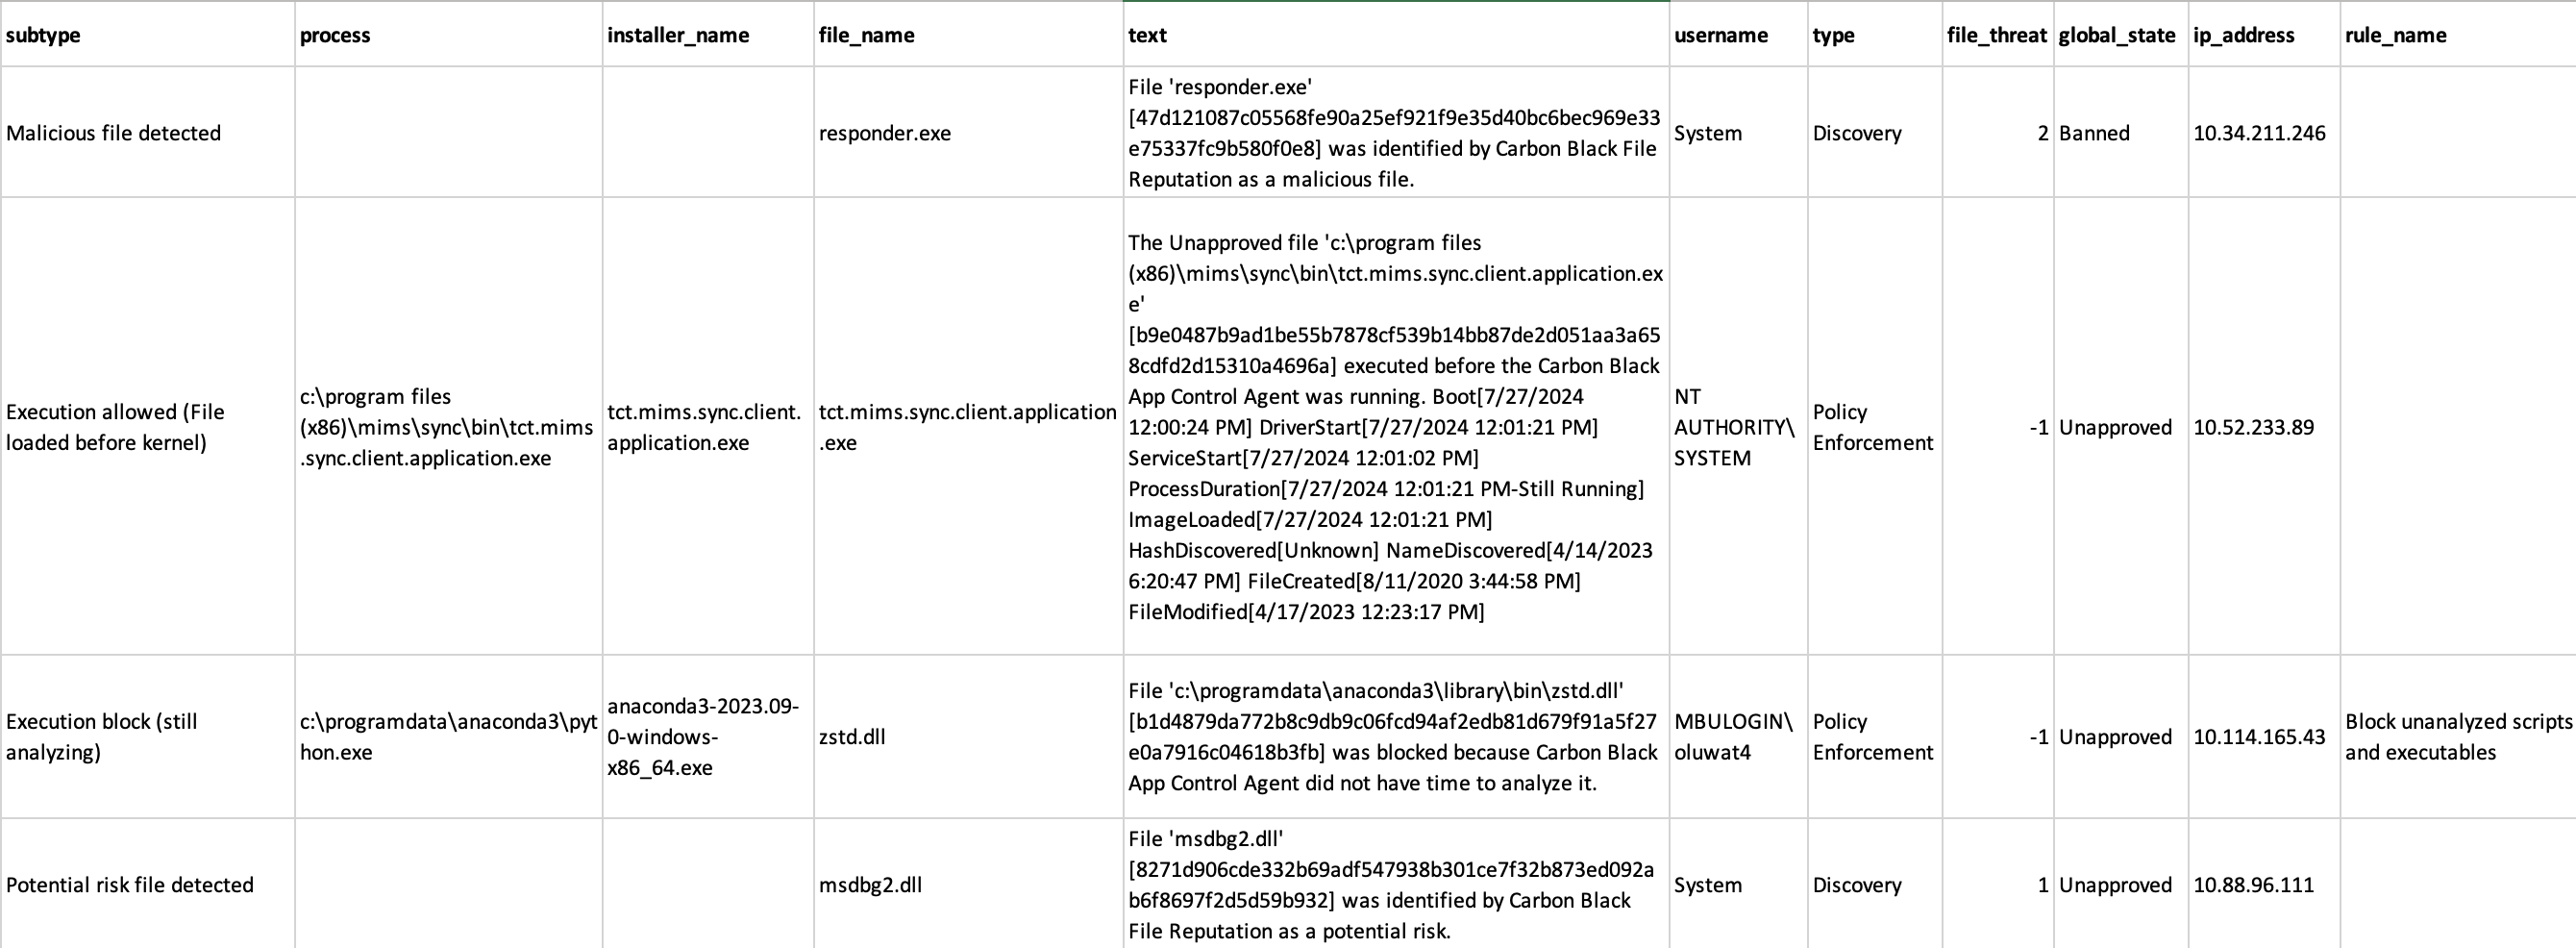
\includegraphics[ width=\textwidth]{../Images/Results.png}
% \end{center}
% \begin{itemize}
%     \item To make results actionable, \_time and IP are included in all results, regardless of their use in the model.
%     \item Results are migrated as .json to CSML1 so the universal forwarder can ingest them to ES.
% \end{itemize}

% \end{frame}